\section{Scientific Paper}

\newpage

\phantomsection
\addcontentsline{toc}{subsection}{1 Introduction}

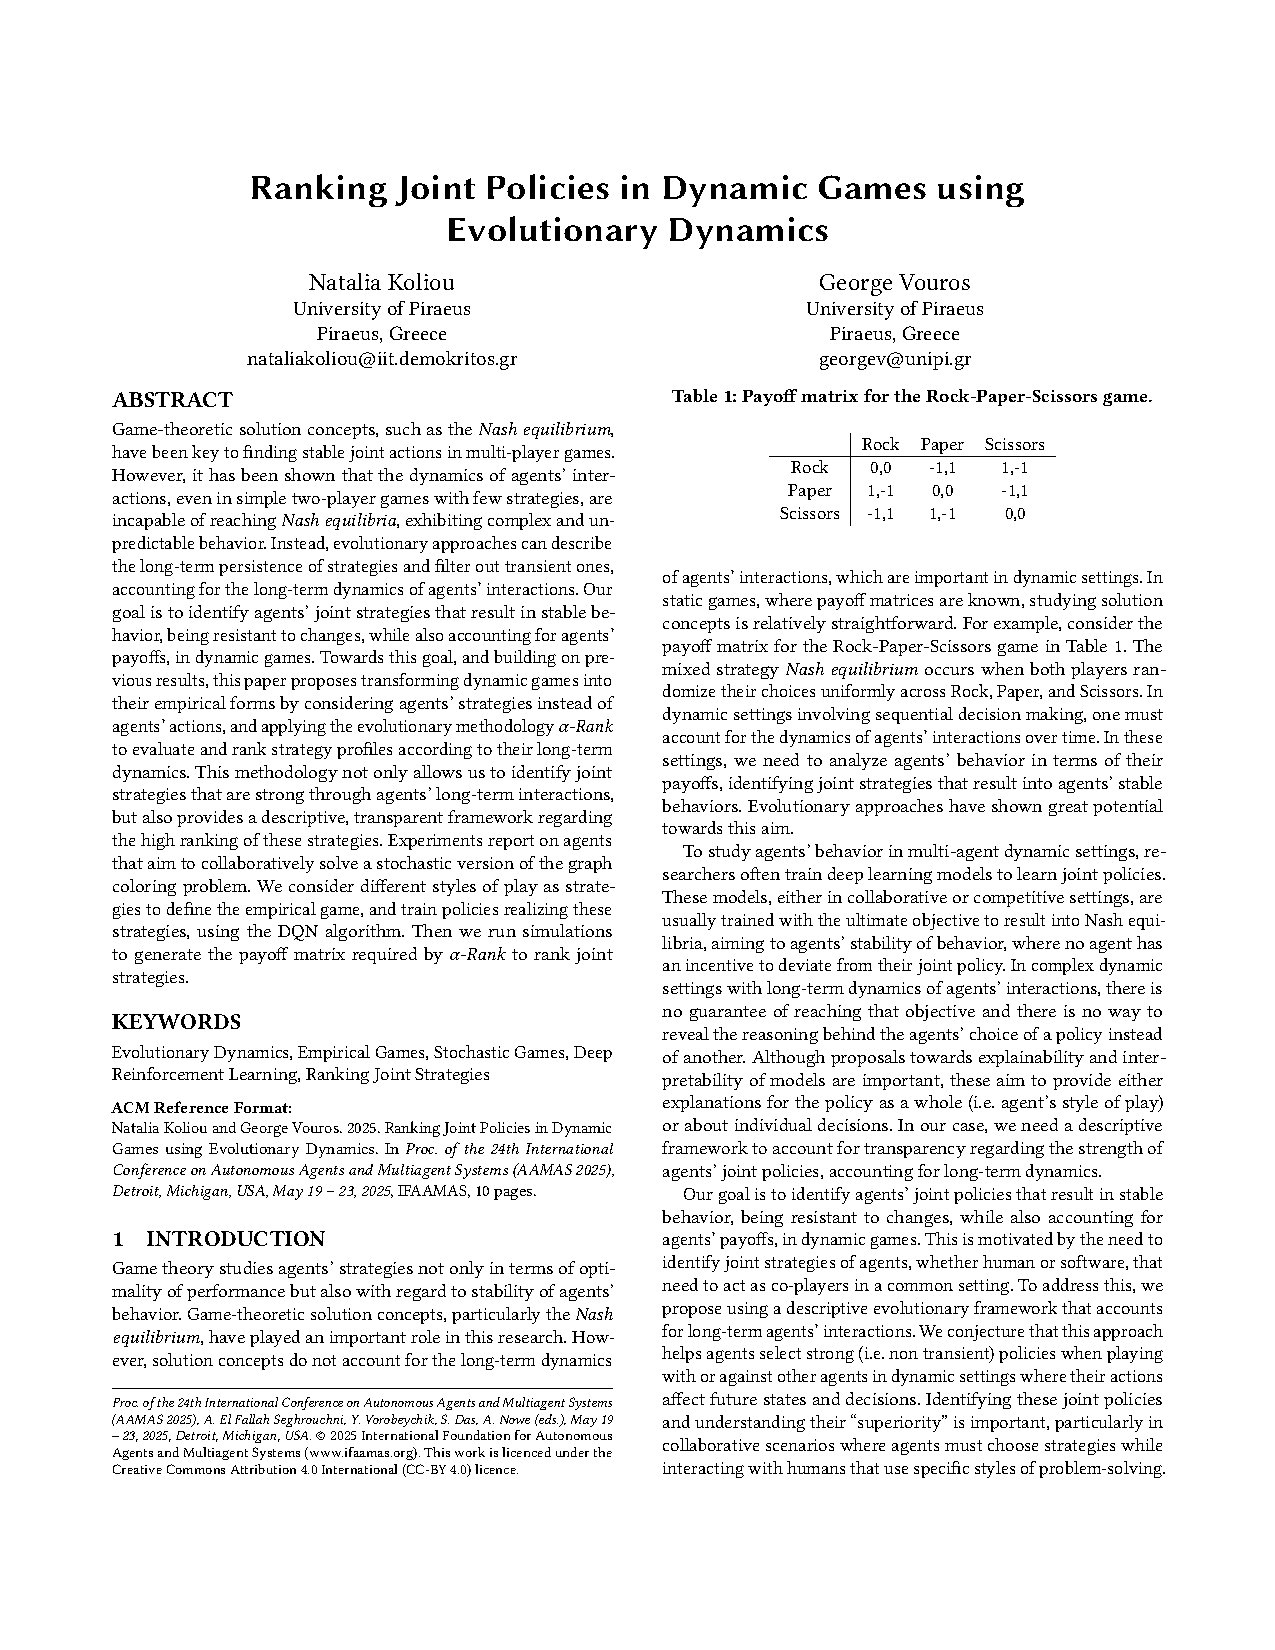
\includepdf[pages=1]{./paper.pdf}

\phantomsection
\addcontentsline{toc}{subsection}{2 Background}

\phantomsection
\addcontentsline{toc}{subsubsection}{2.1 Dynamic Games}

\phantomsection
\addcontentsline{toc}{subsubsection}{2.2 Empirical Analysis and Empirical Games}

\includepdf[pages=2]{./paper.pdf}

\phantomsection
\addcontentsline{toc}{subsubsection}{2.3 The \texorpdfstring{$\alpha$-Rank} Method}

\includepdf[pages=3]{./paper.pdf}

\phantomsection
\addcontentsline{toc}{subsection}{3 Problem Statement}

\phantomsection
\addcontentsline{toc}{subsection}{4 Proposed Method}

\includepdf[pages=4]{./paper.pdf}

\phantomsection
\addcontentsline{toc}{subsection}{5 Experiments and Results}

\phantomsection
\addcontentsline{toc}{subsubsection}{5.1 The Graph Coloring Problem}

\phantomsection
\addcontentsline{toc}{subsubsection}{5.2 Defining the Empirical Game}

\includepdf[pages=5]{./paper.pdf}

\phantomsection
\addcontentsline{toc}{subsubsection}{5.3 Evaluation and Ranking}

\includepdf[pages=6-7]{./paper.pdf}

\phantomsection
\addcontentsline{toc}{subsection}{6 Conclusions}

\includepdf[pages=8]{./paper.pdf}

\phantomsection
\addcontentsline{toc}{subsection}{Appendix A: Empirical Payoff Matrix}

\includepdf[pages=9]{./paper.pdf}

\phantomsection
\addcontentsline{toc}{subsection}{Appendix B: Response Graph}

\includepdf[pages=10]{./paper.pdf}